\section{Experimental Status of Searches for Higgs Boson Pair Production}%
\label{seq:experimental_status}

The experimental status of searches for Higgs boson pair production prior to the
work performed as part of this thesis is summarised in the following. The focus
lies on results by the ATLAS and CMS collaborations obtained using \pp-collision
datasets at $\sqrt{s} = \SI{13}{\TeV}$ during the 2015 and 2016 data-taking
period of the LHC.

The results obtained as part of this thesis will be compared to results of both
collaborations using the \pp-collision datasets recorded from 2015 to 2018 at
the LHC at a later point.


\subsection{Direct Searches for SM Higgs Boson Pair Production}

% https://cms-results.web.cern.ch/cms-results/public-results/publications/HIG-17-030/index.html

\begin{figure}[htbp]
  \centering

  \begin{subfigure}[b]{0.48\textwidth}
    \centering

    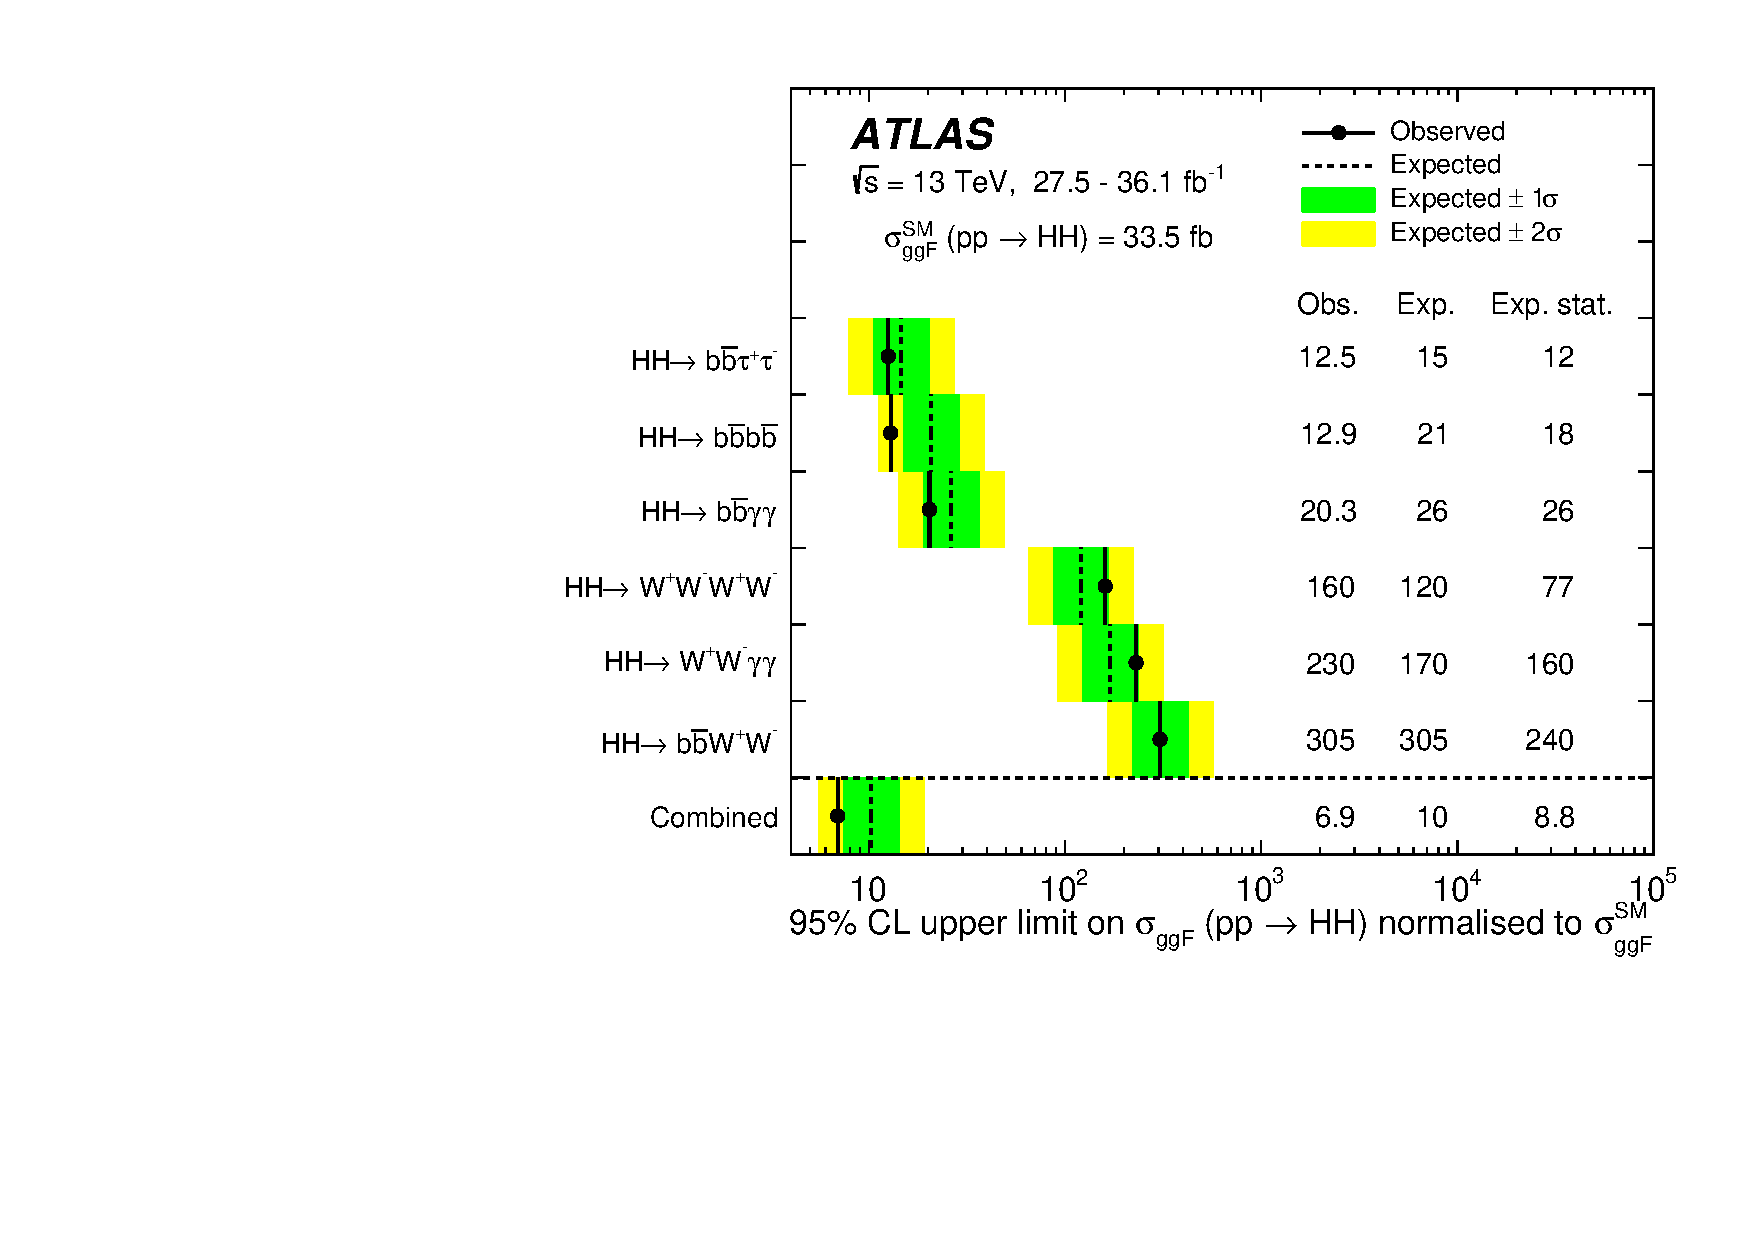
\includegraphics[width=\textwidth]{status/atlas_36ifb}

    \subcaption{The figure is taken from Ref.~\cite{HDBS-2018-58}.}
  \end{subfigure}\hfill%
  \begin{subfigure}[b]{0.48\textwidth}
    \centering

    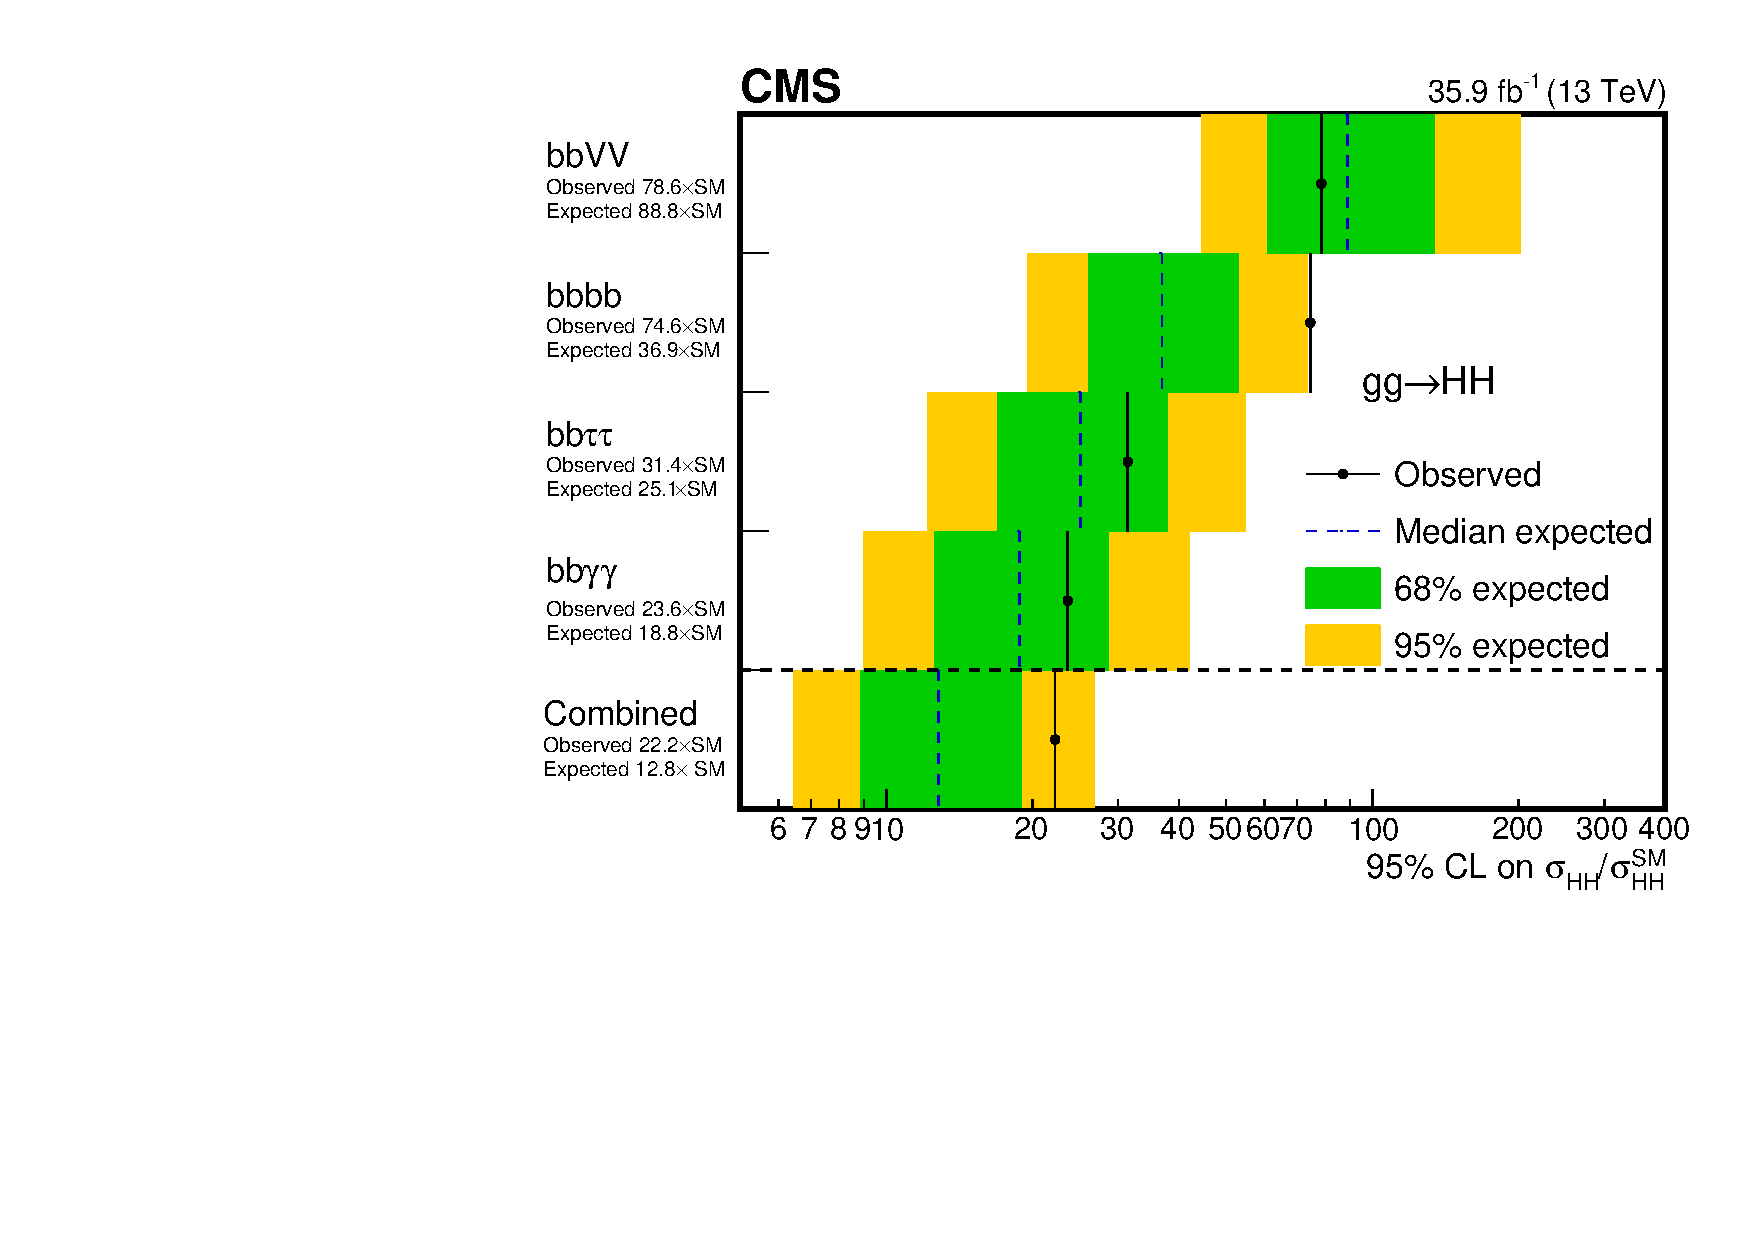
\includegraphics[width=\textwidth]{status/cms_36ifb}

    \subcaption{The figure is taken from Ref.~\cite{CMS-HIG-17-030}.}
  \end{subfigure}

  \caption{Upper limits on the cross-section of SM \HH production via \ggF at
    \SI{95}{\percent} CL by the ATLAS (a) and CMS (b) collaborations. The upper
    limits are normalised to the SM cross section prediction of $\pp \to \HH$
    and given separately for the individual search channels and for the
    statistical combination of all listed channels. The results are based on
    \pp-collision data taken during runs of the LHC in 2015 and 2016.}%
  \label{fig:prior_status}
\end{figure}


\subsection{Constraints on the Trilinear Higgs Boson Self-Coupling}

\begin{figure}[htbp]
  \centering

  \begin{subfigure}[b]{0.48\textwidth}
    \centering

    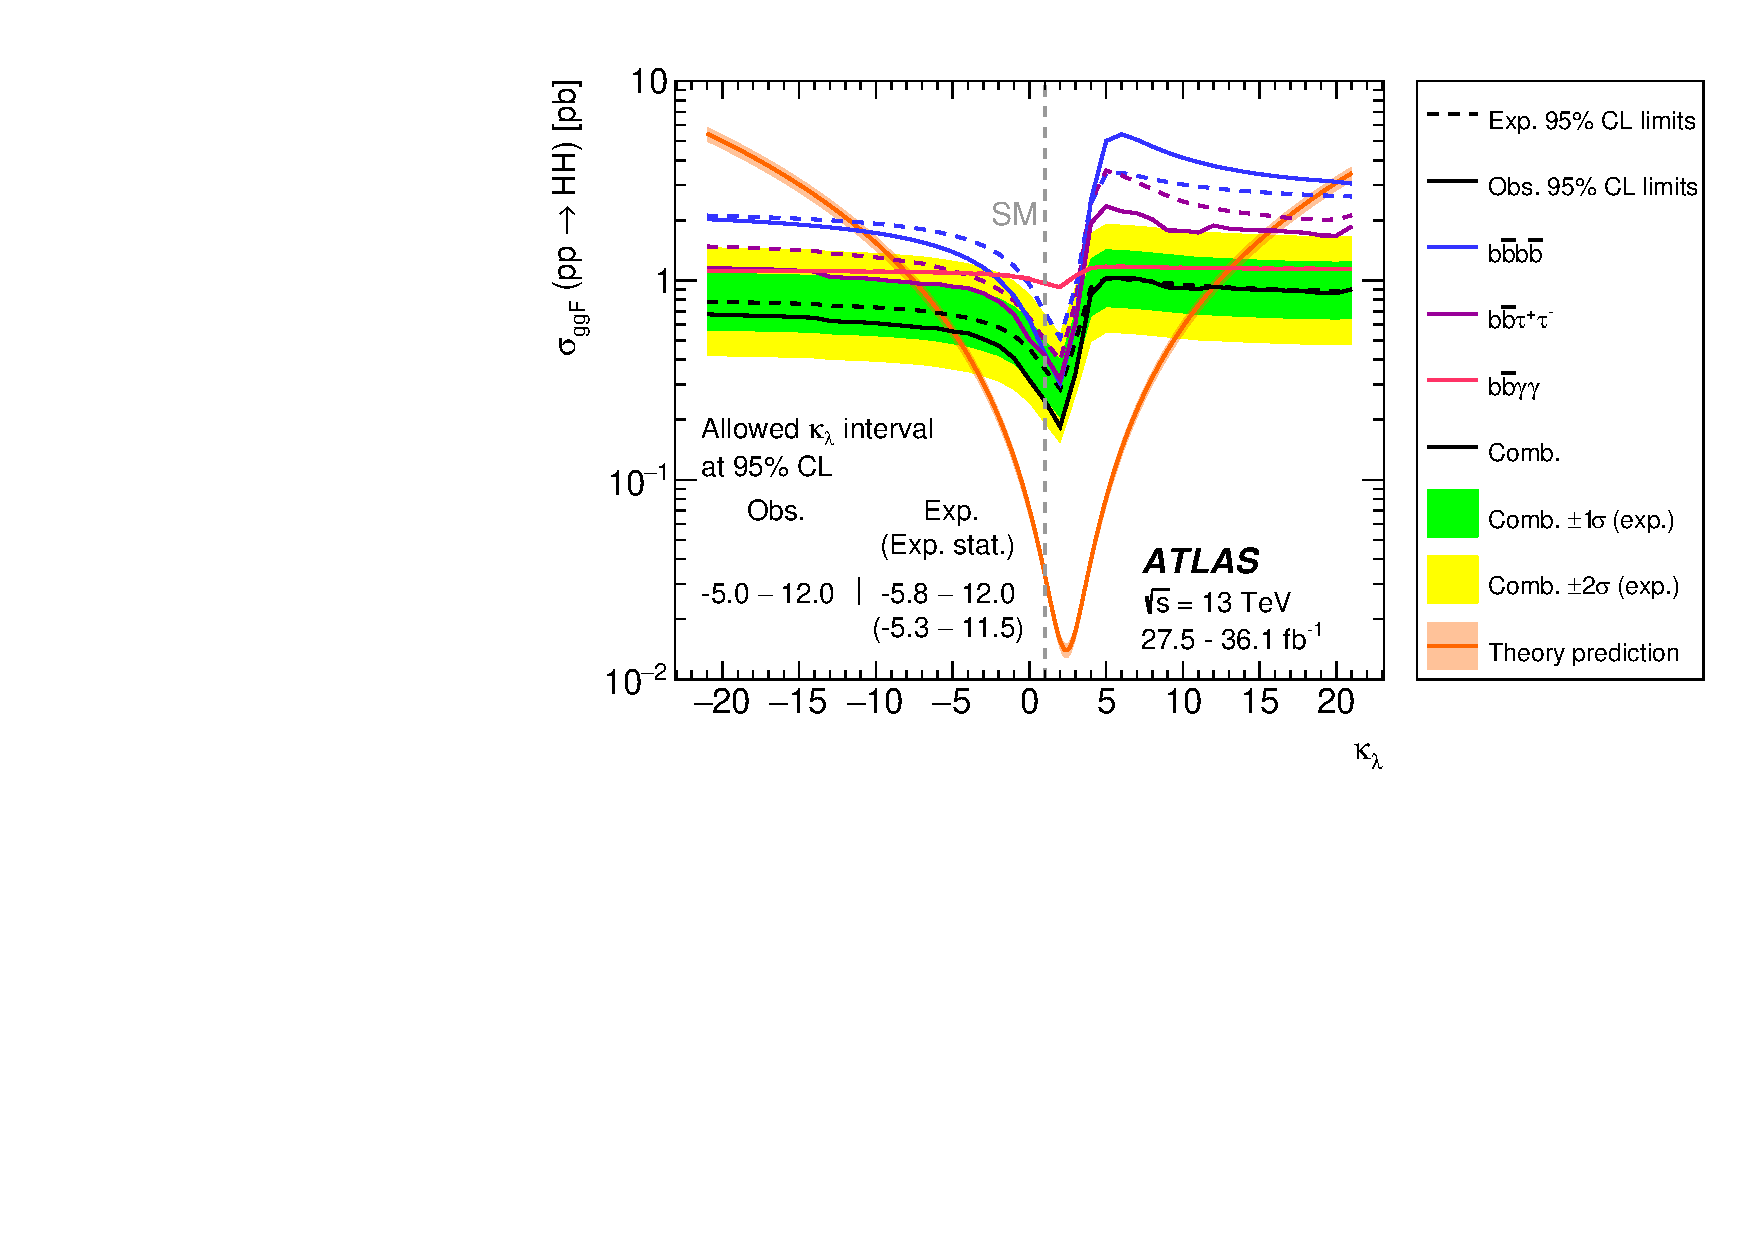
\includegraphics[width=\textwidth]{status/atlas_36ifb_klambda}

    \subcaption{Figure taken from Ref.~\cite{HDBS-2018-58}.}
  \end{subfigure}\hfill%
  \begin{subfigure}[b]{0.48\textwidth}
    \centering

    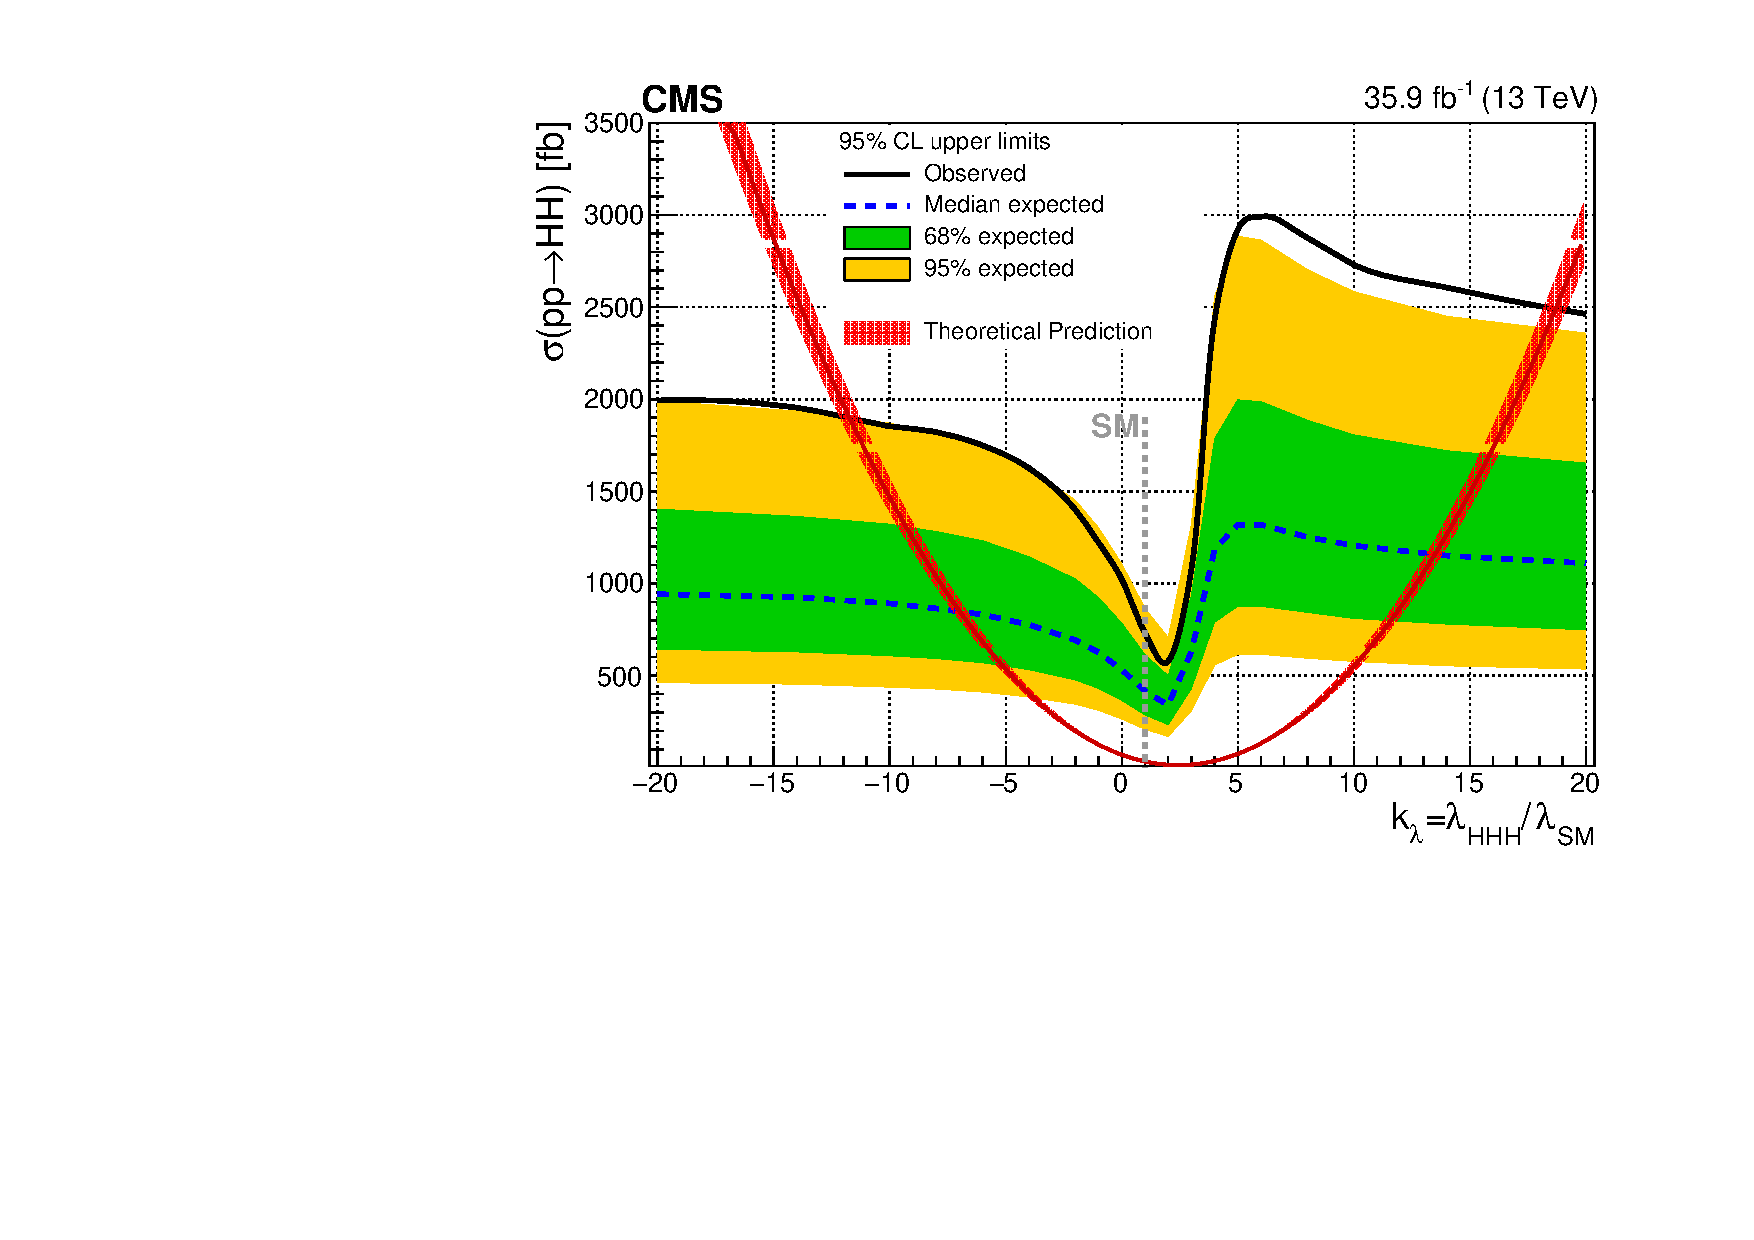
\includegraphics[width=\textwidth]{status/cms_36ifb_klambda}

    \subcaption{Figure taken from Ref.~\cite{CMS-HIG-17-030}.}
  \end{subfigure}

  \caption{Status}%
  \label{fig:prior_status_klambda}
\end{figure}


\subsection{Searches for Resonant Production of Higgs Boson Pairs}


\begin{figure}[htbp]
  \centering

  \begin{subfigure}[b]{0.40\textwidth}
    \centering

    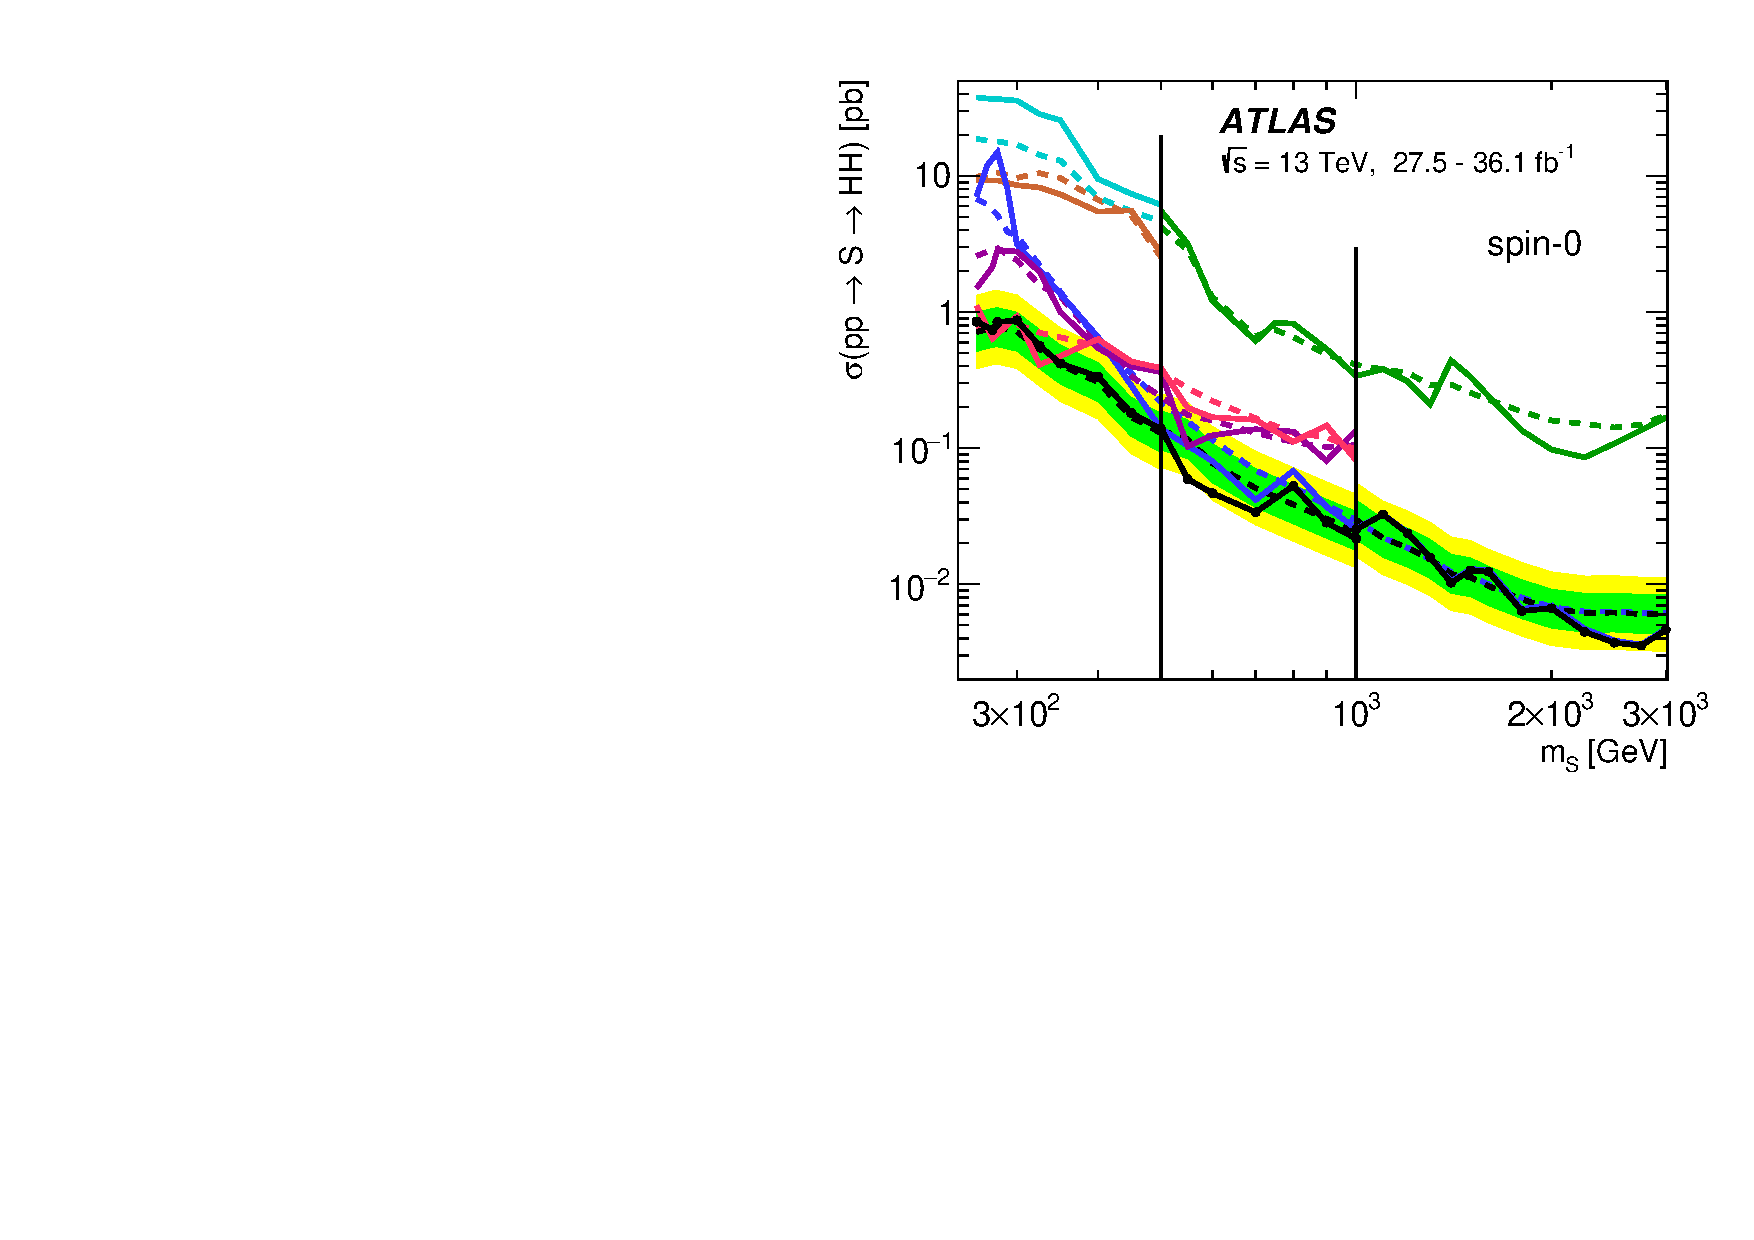
\includegraphics[width=\textwidth]{status/atlas_36ifb_resonant}

    \subcaption{Figure taken from Ref.~\cite{HDBS-2018-58}.}
  \end{subfigure}\hfill%
  \begin{subfigure}[b]{0.56\textwidth}
    \centering

    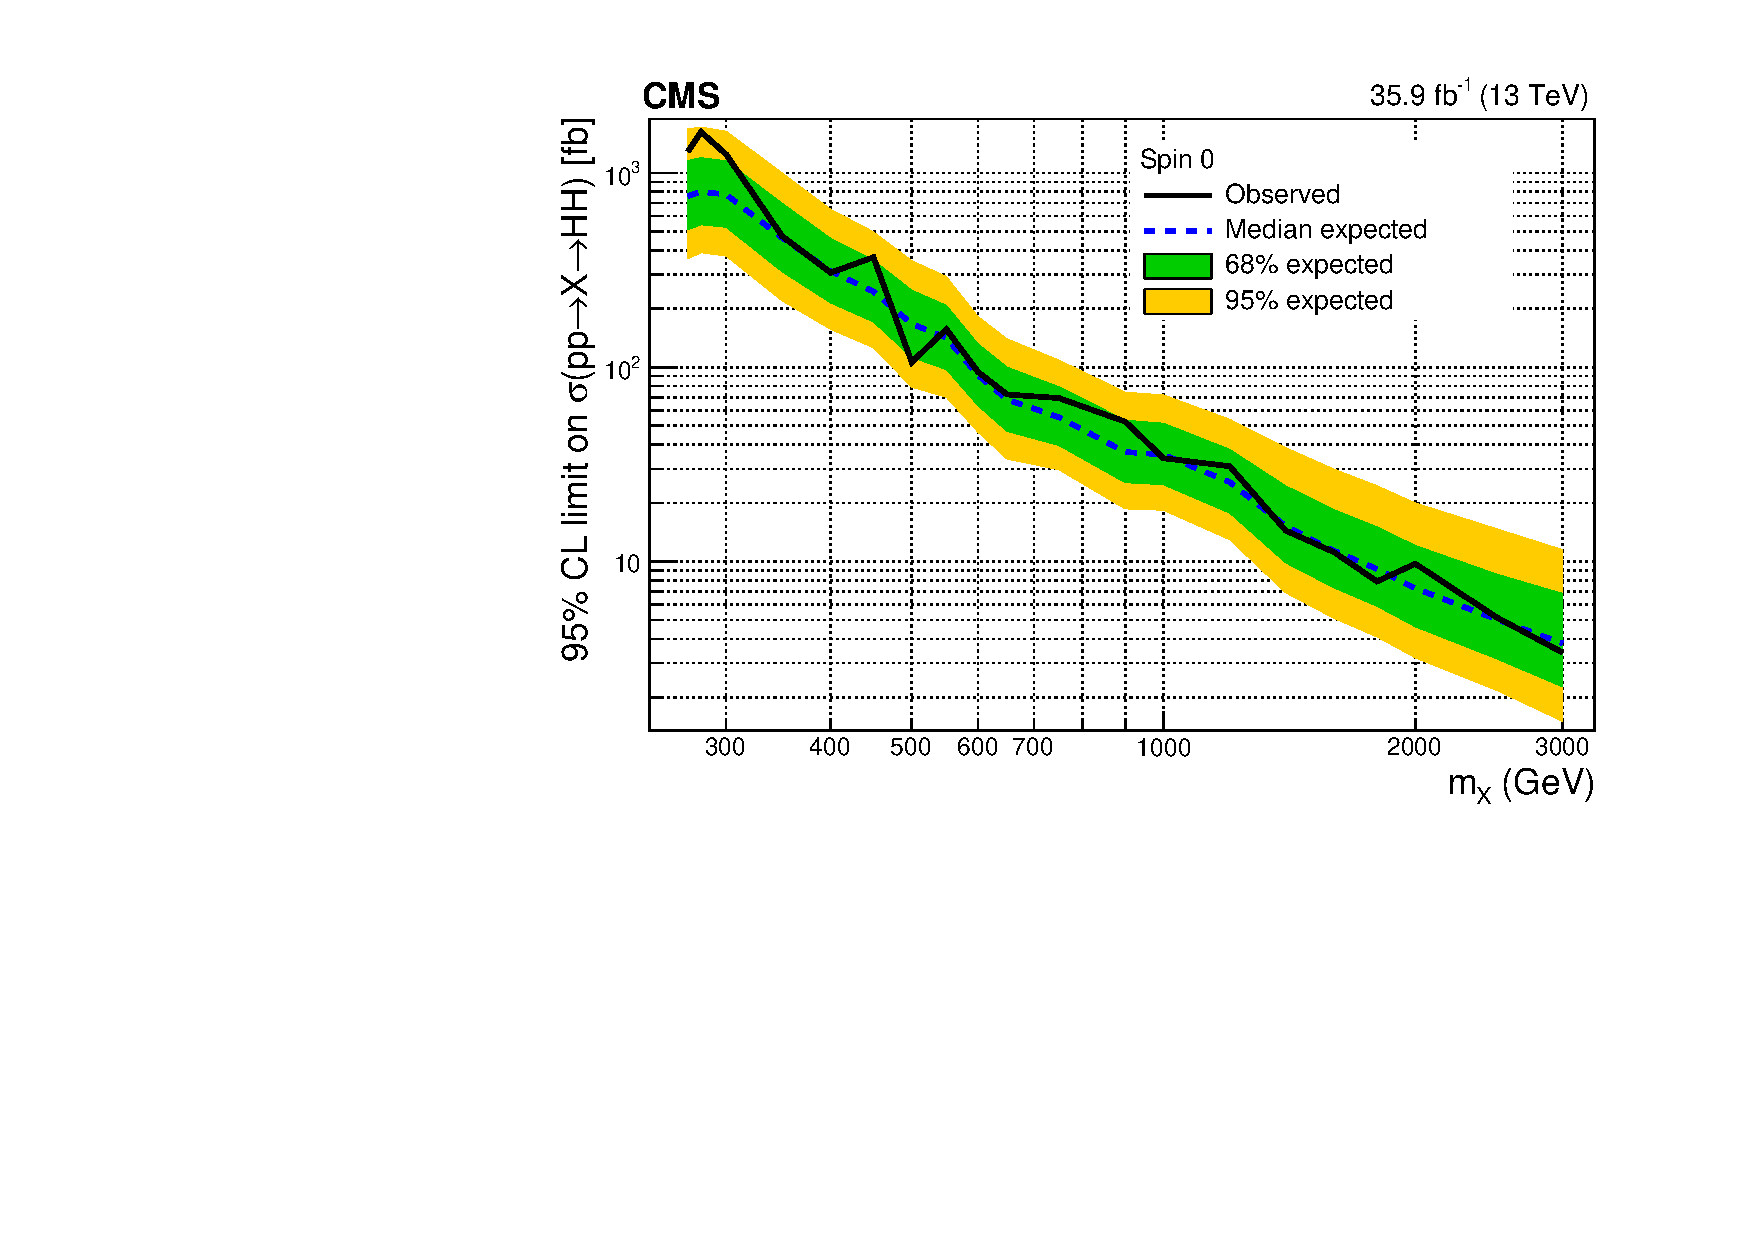
\includegraphics[width=\textwidth]{status/cms_36ifb_resonant}

    \subcaption{Figure taken from Ref.~\cite{CMS-HIG-17-030}.}
  \end{subfigure}

  \caption{Status}%
  \label{fig:prior_status_reso}
\end{figure}


%%% Local Variables:
%%% mode: latex
%%% TeX-master: "../../phd_thesis"
%%% End:
